\section{Logistic Regression}
Logistic Regression is \textbf{Supervised Learning} and subclass \textbf{Classification}.
Logistic Regression is Classification prediction with features.
\subsection{Scenario Admission Decision}
Question is: Will Person be admitted for Masters.
\subsubsection{Data}
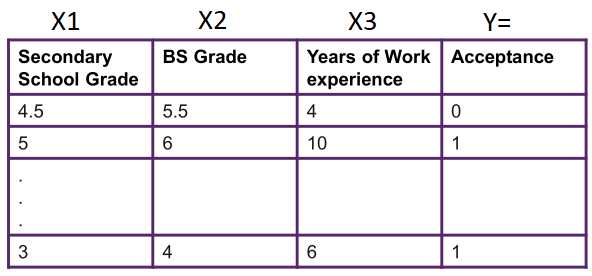
\includegraphics[width=\linewidth]{logistic-reg-data-scen.png}\\
\subsubsection{Joint Probability}
$P(y =1 | x_1 = 4.5, x_2 = 5, x_3 = 5.5)$
\subsubsection{Whole Model}
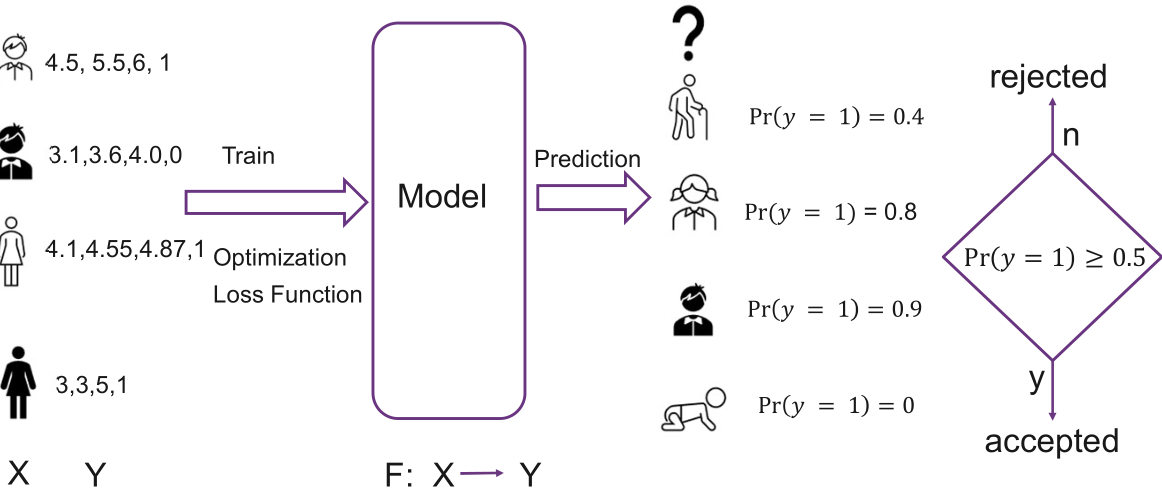
\includegraphics[width=\linewidth]{logistic-regression-example.png}
\subsubsection{Notation}
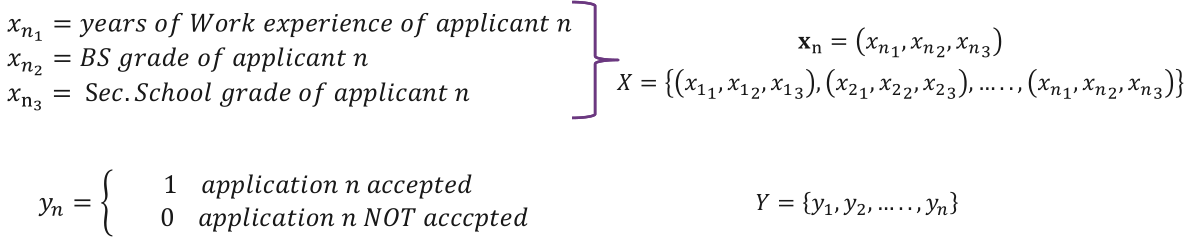
\includegraphics[width=\linewidth]{log-reg-notation.png}\\
N in this case is participant.
Every participant has 3 features and one result $y$.

\subsubsection{Example Probability}
What is the probability that applicant \# 44 is accepted?\\
$Pr(y_{44} = 1 | (x_{44,1},x_{44,2},x_{44,3})) $\\
$ = Pr(y_{44} = 1 | x_{44})$\\
$ = Pr(y = 1 | x)$\\
As soon as the context is set, the notation is minimized.

\subsection{Using Linear Regression}
Not good: Values higher and lower as 1 and 0. Outside of probability.\\
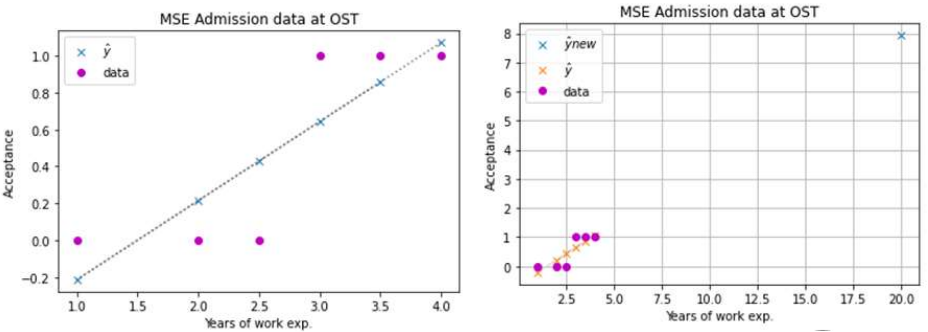
\includegraphics[width=\linewidth]{log-reg-with-lin-reg.png}\\
LR does not work for classification.
MSE forces as wrong solution.

\subsection{Solution}
\subsubsection{The sigmoid function (Model)}
$$p = sigmoid(\hat{y}) = \frac{1}{1 + e^{-\hat{y}}}$$\\
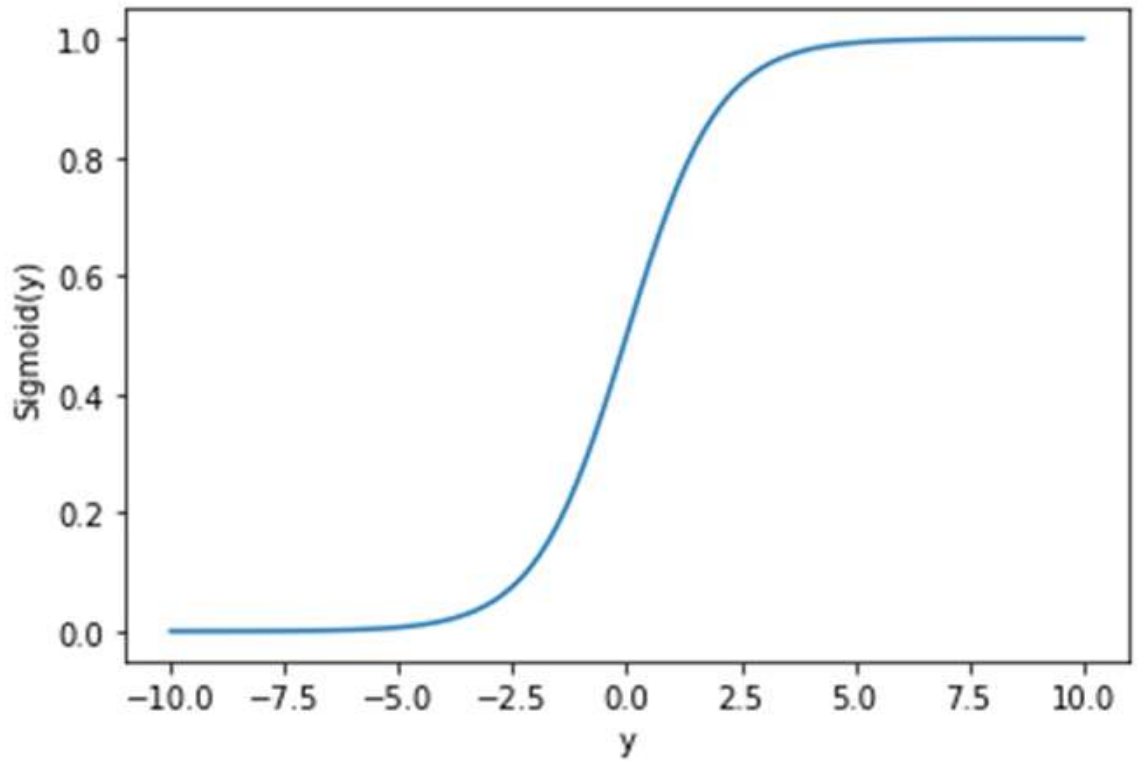
\includegraphics[width=\linewidth]{sigmoid-fun.png}
$$\hat{y} = w_1x_1 + w_2x_2 + w_3x_3\dots$$\\
\textbf{w} is unknown and needs to be learned.

\subsubsection{Maximum Likelihood (Cost-Function (Loss))}
Maximize the likelihood by minimizing cost:\\
$Minimize Cost(W) =$\\
$$\frac{-1}{N}\displaystyle\sum_{i = 1}^{N}(y_i * \log(p_i)) + (1-y_i)*\log(1-p_i)) $$\\
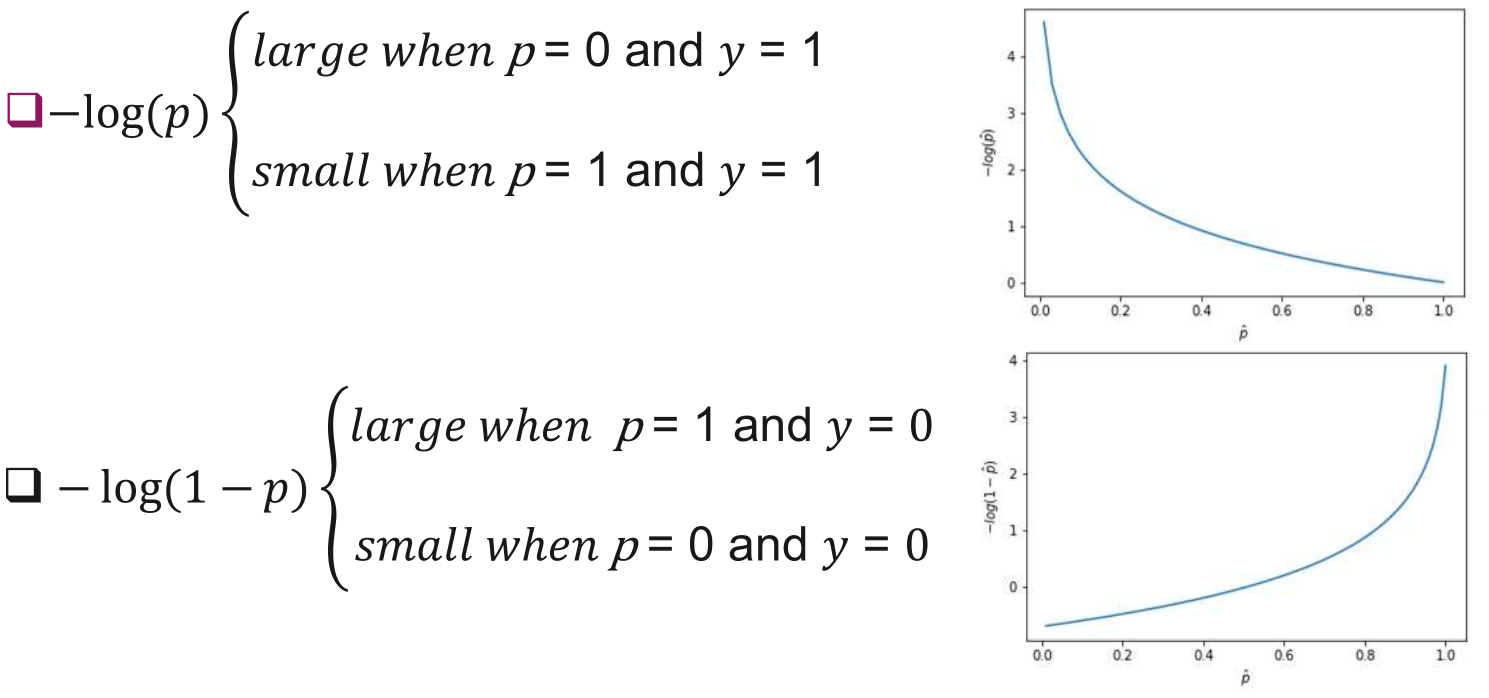
\includegraphics[width=\linewidth]{maximum-liklihood-result.png}